\section{Motor de búsqueda}
\begin{frame}
  \begin{columns}[t]
      \begin{column}{.5\textwidth}
        \tableofcontents[sections={1-2},currentsection]
      \end{column}
      \begin{column}{.5\textwidth}
        \tableofcontents[sections={3-4},currentsection]
      \end{column}
  \end{columns}
\end{frame}

\subsection{Funcionamiento}
\begin{frame}[fragile]{Funcionamiento}

  El funcionamiento en tiempo de búsqueda del programa está regido por la clase Moogle. En esta clase se recibe
  la query como parámetro del método Query y se trabaja con ella.

\pause


\ 


  Primeramente, se guarda la query separada por palabras. Guardamos además en variables auxiliares 
  los valores que resultan de evaluar cada método de la clase Operators. También creamos un array para guardar los
  valores de IDF de cada palabra de la query, un diccionario para relacionar más adelante los scores con el documento
  correspondiente, un diccionario para relacionar cada palabra de la query y la cantidad de veces que se repite en la
  misma. 
  
\end{frame}
  
\begin{frame}[fragile]{Funcionamiento}

  Luego con un foreach llenamos el diccionario poniendo cuántas veces se repite cada palabra en la query.
  En un segundo momento, se crea un primer bucle for para calcular los IDF de las palabras de la query. Para
  ello se utiliza una condicional, de manera que, si la palabra está en algún documento, entonces calculamos su IDF
  y lo multiplicamos por su valor de relevancia y también por la cantidad de veces que está la palabra en la query. 
  En caso contrario pues mantenemos el cero.

\end{frame}

\begin{frame}[fragile]{Funcionamiento}

  Luego de tener los valores de cada palabra de la query, entonces se crea un array donde se va a guardar
  el ranking de los documentos utilizando el método \texttt{GetScore} de la clase \textit{RankingVector}. Después, con un pequeño
  bucle for, le asociamos a cada valor almacenado en score el documento asociado a él (puede haber varios con un
  mismo valor de score, por eso el diccionario recibe como valor una lista). Luego ordenamos el ranking de mayor a
  menor.

\pause


\ 


  Una vez ordenado el ranking, entonces se crea una lista de objetos SearchItem (título, snippet, score) que
  representan cada documento a mostrar en pantalla. 
  
\end{frame}

\begin{frame}[fragile]{Funcionamiento}
  
  Luego existe una condición por si no existen resultados de
  búsqueda:

\pause

\begin{figure}
  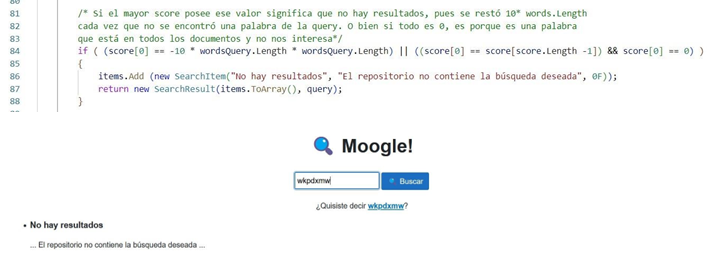
\includegraphics[width=8cm, height=3cm]{img7.png}
\end{figure}

\end{frame}

\begin{frame}[fragile]{Funcionamiento}

  En caso de que sí existan resultados, entonces eliminamos primero los valores repetidos en score, y luego se procede a 
  mostrar los diez documentos con más coincidencias con la búsqueda realizada por el usuario.

\pause


\begin{figure}
  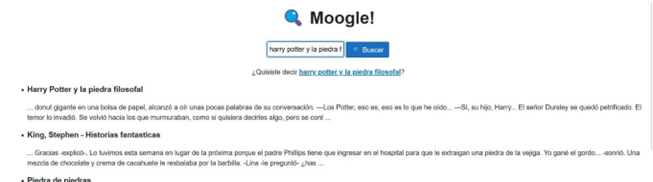
\includegraphics[width=9cm, height=3cm]{img8.png}
\end{figure}


\end{frame}

\begin{frame}[fragile]{Funcionamiento}

En caso de no existir resultados, se le añade lo siguiente al código y se muestra en pantalla:


\pause


\begin{figure}
  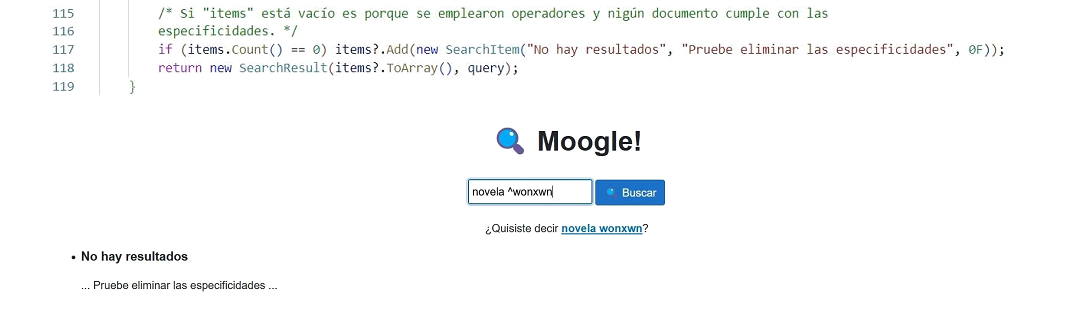
\includegraphics[width=9cm, height=3cm]{img10.png}
\end{figure}



\end{frame}


\subsection{Ver código...}
\begin{frame}[fragile]{Ver código...}

Link de la carpeta \texttt{MoogleEngine}:


\ 


\textcolor{blue}{\underline{\tiny\url{https://github.com/Joel0347/Moogle-/tree/main/Moogle!/MoogleEngine}}}


\ 


\ 


Link de la carpeta \texttt{MoogleServer}:


\ 


\textcolor{blue}{\underline{\tiny\url{https://github.com/Joel0347/Moogle-/tree/main/Moogle!/MoogleServer}}}

\end{frame}
